%--------Anexo 2
%--------Daniel Ochoa John
%--------13/10/2014

\chapter{Estructura del CD}

Junto a este trabajo se adjunta un CD que contiene esta tesis en formato digital, códigos fuente y detalle de experimentos. La Figura \ref{fig:apb-im1} muestra la estructura de directorios del contenido del CD, luego se describen los contenidos de cada carpeta.

\begin{figure}[H]
  \centering
  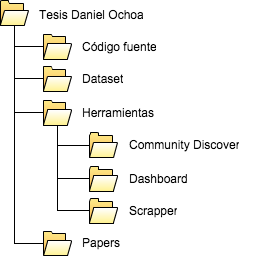
\includegraphics[scale=.5]{images/FiguraB-1}
  \caption{\em Directorios del CD.}
  \label{fig:apb-im1}
\end{figure}

\begin{itemize}
	\item Código fuente: Es una carpeta que contiene el código fuente de RBox 2.0 tal como se puede encontrar en el repositorio de código en bitbucket\footnote{https://bitbucket.org/RodrigoVasquez/recommendation-box}. Es la implementación del \textit{framework} que permite generar sistemas de recomendación en base a la 3-Ontology. La estructura de directorios interna, modo de uso y particularidades de la aplicación pueden encontrarse en el archivo README en la raíz de la carpeta del código fuente.
	\item Dataset: Contiene el \textit{dump} sql de la base de datos de la 3-Ontology que fue utilizada para el análisis. Así mismo, contiene el extenso de los análisis realizados para obtener los resultados.
	\item Herramientas: Contiene todos aquellos componentes desarrollados para complementar el proceso de detección y análisis de comunidades. \newline
	\begin{itemize}
		\item Community Discover: Código del servicio RESTful que permite detectar comunidades. Es una copia fiel del repositorio de código en bitbucket\footnote{https://bitbucket.org/dochoaj/community-discover}. Las instrucciones de uso y precondiciones de instalación están especificadas en el archivo README en la raíz de la carpeta del código fuente.
		\item Dashboard: Código de un dashboard que permite explorar las comunidades detectadas. Es una copia fiel del repositorio de código en bitbucket\footnote{https://bitbucket.org/dochoaj/community-dashboard}. Las instrucciones de uso y precondiciones de instalación están especificadas en el archivo README en la raíz de la carpeta del código fuente.
		\item Scrapper: Código de un scraper que fue utilizado para obtener los datos desde Twitter. Es una copia fiel del repositorio de código en bitbucket\footnote{https://bitbucket.org/dochoaj/3ontology-twitter}. Las instrucciones de uso y precondiciones de instalación están especificadas en el archivo README en la raíz de la carpeta del código fuente.
	\end{itemize}
	\item Papers: Contiene una copia de todos los documentos científicos, a los que fue posible acceder legalmente, y que han sido utilizados como referencia u antecedente de este trabajo de tesis.
\end{itemize}